\documentclass[11pt]{article}
\usepackage{graphicx}
\usepackage{amsmath}
\usepackage{amsfonts}
\usepackage{setspace}
\usepackage{listings} % code inserts
\usepackage{bm} % bold greek math symbols
%\usepackage{fancyvrb}
\usepackage{multirow}
\usepackage[normalem]{ulem} % gives \sout
\usepackage[left=1.0in,top=1.0in,right=1.0in,bottom=1.0in]{geometry}
\usepackage{pslatex}
\usepackage[bookmarks=true,colorlinks=true]{hyperref} 
\usepackage{enumitem}  % adjust item separation

% font
\usepackage[T1]{fontenc}
\usepackage[scaled]{helvet}
\renewcommand*\familydefault{\sfdefault} %% Only if the base font of the document is to be sans serif


% page formatting
%\pdfpagewidth 8.5in
%\pdfpageheight 11in 

\setlength{\parindent}{0pt}
\setlength{\parskip}{10pt}
\setlength{\parsep}{10pt}
%\setlength{\headsep}{0pt}
%\setlength{\topskip}{0pt}
%\setlength{\topmargin}{0pt}
%\setlength{\topsep}{0pt}
%\setlength{\partopsep}{0pt}


% setup headers and footers
%\usepackage{fancyhdr}
%\pagestyle{fancy}   % use default (page numbering on bottom)
%\fancyhead{}        % clear header
%\renewcommand{\headrulewidth}{0in}  % don't show horizontal header bar


% formatting macros
\newcommand{\codeblock}[1]{\vspace{.1in} {\tt #1} \vspace{.1in}}
\newcommand{\comment}[1]{}
\newcommand{\etal}{{\it et al.}}

% reference macros
\newcommand{\figref}[1]{Figure~\ref{#1}}
\newcommand{\supfigref}[2]{Figure~#1\ref{#2}}
\newcommand{\secref}[1]{Section~\ref{#1}}
\newcommand{\appref}[1]{Appendix~\ref{#1}}
\newcommand{\eqnref}[1]{\ref{#1}}
\newcommand{\algref}[1]{Algorithm~\ref{#1}}

\newcommand{\spimap}{{\sf\scshape SPIMAP}}

\DeclareMathOperator*{\argmax}{argmax}
\DeclareMathOperator*{\diag}{diag}
\newcommand{\p}{\partial}
\newcommand{\grad}{\bigtriangledown}
\newcommand{\strike}[1]{\text{\sout{$#1$}}}
\newcommand{\colv}[2]{\left(\begin{array}{c} #1 \\ #2 \end{array}\right)}
\newcommand{\V}[1]{{\bm #1}}
\newcommand{\parent}{\rho}


\newcommand{\gtree}{{\mathbb G}}
\newcommand{\stree}{{\mathbb S}}
\newcommand{\gtop}{T}
\newcommand{\sptop}{S}
\newcommand{\recon}{R}


\bibliographystyle{plain}



%=============================================================================
\begin{document}


%=============================================================================
% TITLE PAGE

\begin{center}
{\Huge \bf 
SPIMAP: Species Informed Maximum A Posteriori Gene Tree Reconstruction
}

\vspace{.2in}

{\LARGE 
Documentation for the SPIMAP software package
}

{\LARGE \today}


\vspace{.5in}

{\bf Author:} Matthew D. Rasmussen (rasmus@mit.edu, matt.rasmus@gmail.com) \\
{\bf Software website:} http://compbio.mit.edu/spimap

\vspace{.1in}

{\bf citation}: \\
Matthew D. Rasmussen and Manolis Kellis.
{\it A Bayesian Approach for Fast and Accurate Gene Tree Reconstruction}.
Molecular Biology and Evolution. 2010. doi: 10.1093/molbev/msq189

\end{center}

\newpage

\tableofcontents

\newpage

%=============================================================================
\section{Introduction}

This documention is currently under development and will be regularly 
updated with more information about the \spimap\ software package.


%=============================================================================
\section{Programs}

%=========================================
% PARAMS FIGURE
\begin{figure}
\begin{center}
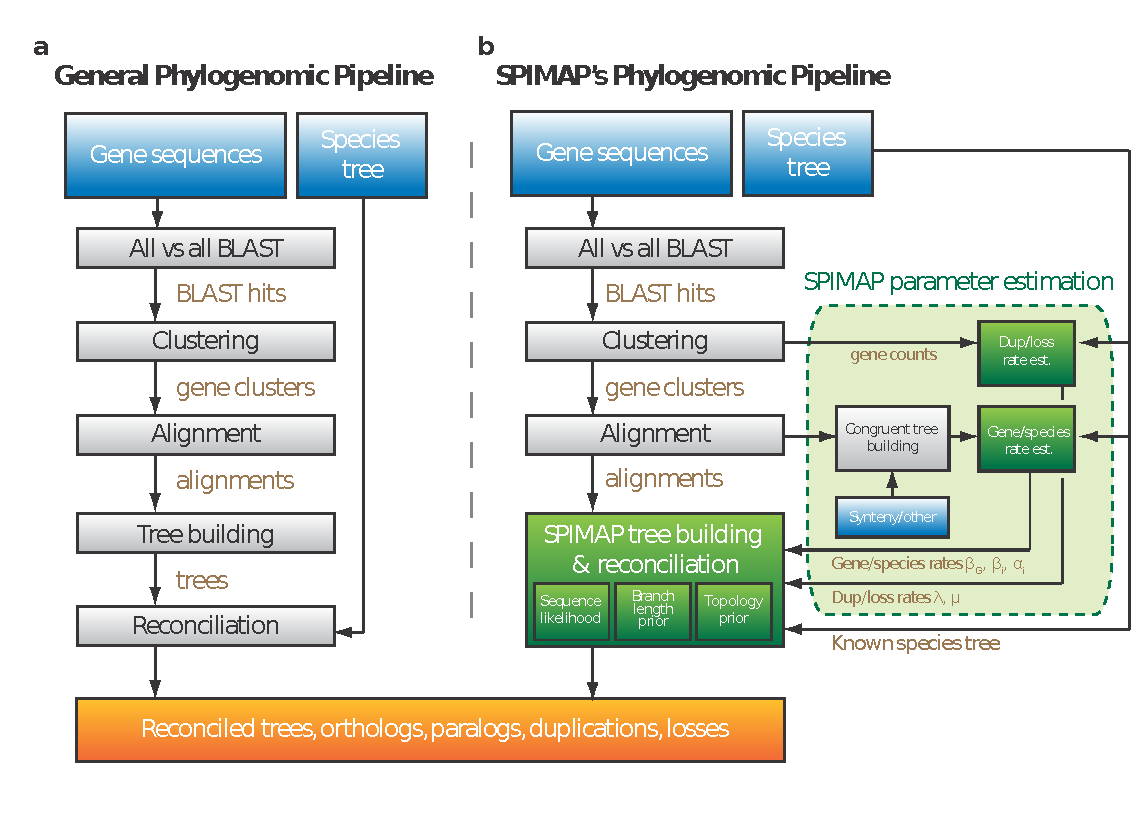
\includegraphics[width=5.5in]{figures/pipeline.pdf}
\vspace{-.4in}
\end{center}

\caption{{\bf Computational pipeline for the SPIMAP software package.}
 (a) The typical phylogenomic pipeline consists of several common
 steps, although particular implementations may vary.  The pipeline
 input is the set of all gene sequences across several species and the
 known species tree relating the species (blue boxes).  Gene sequences
 are then compared across species and clustered according to their
 sequence similarity, resulting in a set of homologous gene families.
 A multiple sequence alignment is then constructed for each gene
 family, followed by phylogenetic reconstruction of each aligned
 family to produce gene trees.  Each gene tree is then reconciled to
 the known species tree in order to infer orthologs, paralogs, and
 gene duplications and loss events, which are the pipeline outputs
 (orange box).  \newline (b) Our phylogenomic pipeline follows similar
 steps, except that \spimap\ includes a model parameter estimation
 step (dashed light green box).  Using per-species gene counts in the
 gene clusters, the {\tt spimap-train-duploss} program
 (\secref{sec:prog:spimap-train-duploss}) learns duplication and loss
 rates ($\lambda$ and $\mu$).  Using a subset of trusted orthologous
 alignments supported by synteny or other information and congruent to
 the species tree, the {\tt spimap-train-rates} program
 (\secref{sec:prog:spimap-train-rates}) learns gene- and
 species-specific substitution rates ($\beta_G, \V{\alpha},
 \V{\beta}$). These learned evolutionary parameters are then
used by the {\tt spimap} program (\secref{sec:prog:spimap}) to perform
 gene tree building and reconciliation simultaneously (dark
 green box). }
\label{fig:pipeline}
\end{figure}

%=============================================================================
\subsection{spimap}
\label{sec:prog:spimap}

The main \spimap\ algorithm is implemented in the {\tt spimap} program.
The purpose of this program is reconstruct gene trees from DNA alignments.
Accurately reconstructing gene trees is a challenging problem.  \spimap's
strategy is to more accurately reconstruct gene trees by using additional 
information learned from the species tree and the genome.  

This genome-wide information is captured in two sets of parameters 
that the {\tt spimap} program needs.  The first set are gene duplication and
loss rates ($\lambda$ and $\mu$).  You can either specify these rates 
based on previously performed studies, or you can use the
{\tt spimap-train-duploss} program (\secref{sec:prog:spimap-train-duploss})
to learn them from gene counts.

The second set of parameters needed by {\tt spimap} are substitution rate
parameters ($\beta_G$, $\V{\alpha}$, $\V{\beta}$).  These are estimated
from a small subset of trusted purely orthologous gene trees.  Once these
parameters are learned, they can be used to aid in the reconstruction
of more difficult paralogous families.  This package provides the
{\tt spimap-train-rates} program (\secref{sec:prog:spimap-train-rates}),
which can estimate these parameters.

The \figref{fig:pipeline} illustrates a computational pipeline for how
the three programs ({\tt spimap}, {\tt spimap-train-duploss}, and 
{\tt spimap-train-rates}) work together.  Additionally, this package also
includes several other helper programs that can prepare data sets for 
training (see {\tt spimap-prep-duploss} \secref{sec:prog:spimap-prep-duploss}
and {\tt spimap-prep-rates} \secref{sec:prog:spimap-prep-rates}).


\subsubsection{spimap arguments}

{\bf Main arguments}

{\tt -a,--align  <alignment fasta>}

Use this argument to specify the DNA alignment that you would to use
for reconstructing a gene tree.  The file should be in FASTA format
(\secref{sec:file:align}).


{\tt -S,--smap  <species map>}

Use this argument to specify which species each gene belongs.  {\tt
<species map>} should be a file in *.smap format
(\secref{sec:file:smap}).

{\tt -s,--stree  <species tree>}

Use this argument to specify known species tree specified in a file
{\tt <species tree>} written in newick format
(\secref{sec:file:stree}).

{\tt -p,--param  <params file>}

Use this argument to specify the \spimap substitution rate parameters
($\beta_G$, $\beta$, $\alpha)$ written in the *.param file format
(\secref{sec:file:params}).  This file is generated by {\tt
spimap-train-rates} (\secref{sec:prog:spimap-train-rates}).

{\tt -o,--output  <output filename prefix>}

Use this argument to specify a prefix for all of the output files.  By 
default the prefix is ``spimap'' (e.g. ``spimap.tree'', ``spimap.recon'', 
``spimap.log'').  The prefix can also specify a different output directory.

{\tt -r,--recon}

With this argument \spimap\ will output the reconciliation found to the 
file ``<output filename prefix>.recon'' written in the *.recon format 
(\secref{sec:file:recon}).


{\bf Sequence evolution model arguments}

{\tt -k,--kappa  <transition/transversion ratio>}

Use this argument to specify the transition/transversion ratio $\kappa$
for the HKY sequence model.  By default $\kappa$ will be estimated 
from the alignment.

{\tt -f,--bgfreq  <A freq>,<C ferq>,<G freq>,<T freq>}

Use this argument to specify the background base frequency for the 
HKY sequence model.  By default these frequencies are estimated from the
alignment.


{\bf Dup/loss evolution model arguments}

{\tt -D,--duprate  <duplication rate>}

This specifies the gene duplication rate.  Commonly, this should be 
specified in units of duplications/gene/million years.  See 
\secref{sec:file:stree} for a discussion of the unit of time.

{\tt -L,--lossrate  <loss rate>}

This specifies the gene loss rate.  Commonly, this should be 
specified in units of loss/gene/million years.  See 
\secref{sec:file:stree} for a discussion of the unit of time.


{\bf Search arguments}

{\tt -i,--niter  <number iterations>}

This specifies the number of iterations \spimap\ should search for the 
MAP gene tree.

{\tt --quickiter  <quick iterations>}

This specifies the number of subproposals (default=50) for each main 
search iteration.  Choosing a number between 100-1000 usually increases
search efficiency, therefore allowing one to use fewer main iterations 
(``-i'').

{\tt -b,--boot  <number bootstraps>}

Use this argument to perform bootstrapping.  The alignment will be resampled
with replacement {\tt <number bootstrap>} times and a gene tree will be 
reconstructed for each sample.

{\bf Information arguments}

{\tt -V,--verbose  <verbosity level>}

You can adjust the amount of logging/debugging information that \spimap\ 
displays by adjusting this argument (0=quiet, 1=low, 2=medium, 3=high)


{\tt --log  <log filename>}

This specifies a different file for saving log information.
Use ``-'' to display on stdout (standard output).

{\tt -v,--version}

When given, \spimap\ will display version information.

{\tt -h,--help}

When given, \spimap\ display help information.


%=============================================================================
\subsection{spimap-prep-duploss}
\label{sec:prog:spimap-prep-duploss}

XXX

%=============================================================================
\subsection{spimap-train-duploss}
\label{sec:prog:spimap-train-duploss}

XXX

%=============================================================================
\subsection{spimap-prep-rates}
\label{sec:prog:spimap-prep-rates}

XXX

%=============================================================================
\subsection{spimap-train-rates}
\label{sec:prog:spimap-train-rates}

XXX

%=============================================================================
\subsection{spimap-sim}
\label{sec:prog:spimap-sim}

XXX



%=============================================================================
\section{Preparing your data set}
\label{sec:prepar}

\paragraph{Restrictions on gene IDs and species IDs.}  Due to the
file formats that \spimap\ uses, there as several restrictions on what IDs
are allowed.  Many of these restrictions are common for other similar
phylogenetic software.  The safest IDs follow these restrictions:
\begin{enumerate}[itemsep=0pt,topsep=0pt]
\item the first and last characters of the ID are a-z A-Z 0-9 \_ - .
\item the middle characters can be a-z A-Z 0-9 \_ - . or the space character ' '
\item the ID should not be purely numerical characters 0-9
\item the ID should be unique within a gene tree or within a species tree
\end{enumerate}

Space characters are discouraged from gene IDs and species IDs since
they will probably cause problems with other bioinfomatic software
that you may use (although \spimap\ can handle spaces).  Characters
such as parentheses ``(`` ``)'' and colons ``:'' are not allowed
because the newick file format (see \secref{sec:file:stree}) uses these
characters for describing the structure of the tree.

It is also easier to use gene IDs that have a prefix or suffix that indicates
the species ID.  For example ``human\_HOXC5'' is a human gene.  This is not
a requirement, but it does make preparing a gene to species mapping 
file (*.smap) easier (see \secref{sec:file:smap}).



%=============================================================================
\section{File formats}

%=============================================================================
\subsection{Sequence alignment format (*.align)}
\label{sec:file:align}

\spimap\ uses the FASTA file format
(\url{http://en.wikipedia.org/wiki/FASTA\_format}) for sequences
alignments.  The file extension is not important and many different 
extensions are in common use (*.fa, *.mfa, *.fasta, *.align).

Each line starting with ``>'' indicates a gene name
(\figref{fig:align}).  Note, the entire line after the ``>'' is used as the
gene name.  The gene's sequence is given on the following
lines and it may be wrapped to any number of columns (or not wrapped at
all).  Gaps in the alignment are represented with the ``-'' character.

At this time (version 1.1), \spimap\ can only use DNA sequences.  The
sequence can be in both upper case and lower case (\spimap\ ignores
case) and degeneracy codes can be used (``NnRrYyWwSsKkMmBbDdHhVv''),
however at this time \spimap\ treats all degeneracies as completely
missing data (``N'').  Gaps ``-'' are also treated as missing data.


%=========================================
% ALIGN FIGURE
\begin{figure}
\begin{center}
\footnotesize
\begin{lstlisting}[frame=tblr]
>KLLA0C08239g
ATGAGTCTCAAACGTGTAGTTGTCACTGGTCTTGGGGCCTACACGCCCCTTGGTTCTACAGTTTCAAAGTCTTGGGCAGG
TTTGCTT---GCTGCTAAGCAATCACTAATACCCTTAGATGCTTTCTACAACAGAGAA---GACTTTGCAAAAGTGAAAA
AGTTGGTCCCACTAGATACAGCAGTGAGTAGGTTACAT------------------------------------------
>ADL072C
---ATGCATCCCCGAGTGGTCGTGACCGGCATTGGGTGCTATACTCCTCTGGGGCCGTCGCTAGCCCAGTCTTGGAAGGA
GCTGTTG---CGAGGGACGAGCGGCCTTGTCAGGCTGCAAGATCTGGCAGAGTACGAGGGCGATTACAAACCACTGTCGA
GGCTTATATCCGGTGATCTTCGAGTCGGGAAAGTTGGATTTGAG------------------------------------
>kwal_5828
---ATGACTTCCAGAGTCGTTGTTACTGGGCTTGGTGCTATCACTCCACTTGGGAGGACTGTTTCCGAGTCATGGAGAGC
TTTATTG---GCAGGCAAGTCCGGAATTCGTCCCATTCGCGATCTTCCC------------AATGCTAAAAGCTACGAAG
GACACTGTCCTGCATCTGTTGCCGTTGCAGACATTCCTGATTTC------------GATCCA------------------
\end{lstlisting}
\end{center}

\caption{{\bf Example *.align file.} Three gene DNA sequences
are given, each with 240 sites.}
\label{fig:align}
\end{figure}


%=============================================================================
\subsection{Species tree file format (*.stree)}
\label{sec:file:stree}

Species trees should be specified using the Newick file format.  See
\url{http://en.wikipedia.org/wiki/Newick\_format} for details.  Beyond
the newick format, \spimap\ has only a few additional requirements.
First, the species names given in the species tree should match those
given in the SMAP file (\secref{sec:file:smap}).  Second, the branch
lengths of the species tree should be expressed in units of time
(\figref{fig:stree}).  Any unit of time can be used (e.g. millions of
years, generations, relative units, etc).  The only requirement is
that the duplication and loss rates are also expressed in compatible
units.  Therefore, if branch lengths are in {\em millions of years},
the duplication rate (specified by {\tt spimap}'s ``-D'' option)
should be in units of duplications/gene/{\em million years}.

\paragraph{Naming ancestral nodes.}
\spimap\ also supports naming ancestral nodes in the species tree using
the newick format.  For example, the parental node of {\tt human} and 
{\tt chimp} can be named {\tt primate} using the following syntax:

\begin{lstlisting}
((human:5,chimp:5)primate:70,mouse:75)mammal;
\end{lstlisting}

If ancestral nodes are named, they will be used in the output of the 
reconciliation mapping (\secref{sec:file:recon}).



%=========================================
% STREE FIGURE
\begin{figure}
\begin{center}

\begin{minipage}{2in}
\tiny
\begin{lstlisting}[frame=tblr]
(((((((scer:7.061760,
       spar:7.061760
      )n7:4.999680,
      smik:12.061440
     )n6:5.970600,
     sbay:18.032040
    )n5:52.682400,
    cgla:70.714260
   )n4:7.220700,
   scas:77.934960
  )n3:23.181480,
  (
   (
    agos:78.553260,
    klac:78.553260
   )n9:10.434960,
   kwal:88.988220
  )n8:12.128400
 )n2:78.883560,
 (
  (
   (
    calb:41.275620,
    ctro:41.275980
   )n12:29.632860,
   (
    cpar:52.323120,
    lelo:52.323120
   )n13:18.585720
  )n11:31.149540,
  (
   (
    cgui:75.615840,
    dhan:75.615840
   )n15:14.006880,
   clus:89.622720
  )n14:12.435660
 )n10:77.941620
)n1;
\end{lstlisting}
\end{minipage} \hfill \begin{minipage}{4in}
\hspace{.5in}
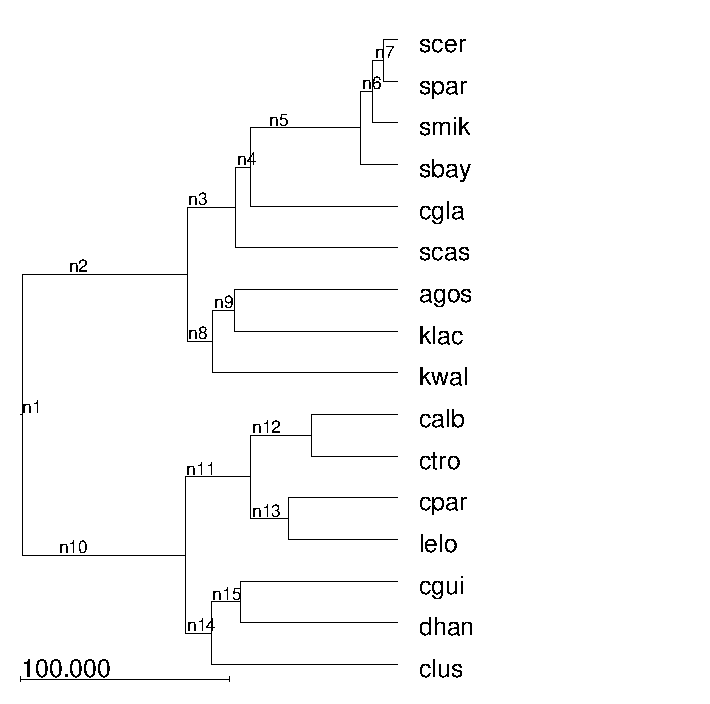
\includegraphics[width=4in]{figures/fungi-stree.pdf}
\end{minipage}


\end{center}

\caption{{\bf Example *.stree file and corresponding tree.} This file
(left) specifies the species tree (right) using the newick file
format.  Branch lengths should be expressed in units of time
(e.g. millions of years).  Ancestral nodes can also optionally be
named (the names ``n1'', ``n2'', etc are used in this example).}
\label{fig:stree}
\end{figure}



%=============================================================================
\subsection{Gene to species name mapping file format (*.smap)}
\label{sec:file:smap}

\spimap\ uses a special file format ({\tt *.smap}) to specify which
genes belong to which species. Each line contains two tab-delimited
fields: 
\begin{enumerate}[itemsep=0pt,topsep=0pt]
\item pattern matching a gene ID
\item species ID
\end{enumerate}

Only 3 types of gene ID patterns are supported.  The pattern can
either be an exact matching string, a prefix (denoted {\tt "text*"}),
or a suffix (denoted {\tt "*text"}).  The "*" is the only special
wildcard character.

The species ID should be the same as those used in the species tree.
All patterns and IDs are case-sensitive.

When mapping a gene ID to a species ID all exact matches are
processed first.  If no exact match is found, the patterns are then
processed in the same order as they appear in the file until a match
is found. For example in the SMAP file given in \figref{fig:smap}, the
gene ID {\tt "YALI123"} should match the species {\tt "ylip"}, instead of
{\tt"scer"}, because the pattern {\tt "YALI*"} occurs before {\tt
"Y*"}.


%=========================================
% SMAP FIGURE
\begin{figure}
\begin{center}
\footnotesize
\begin{lstlisting}[frame=tblr]
A*      agos
orf19*  calb
CDUG_*  cdub
CAGL*   cgla
IPF_*   cgla
CGUG_*  cgui
sbay_*  sbay
scas_*  scas
smik_*  smik
spar_*  spar
SCP*    spom
YALI*   ylip
Y*      scer
Q*      scer
\end{lstlisting}
\end{center}

\caption{{\bf Example *.smap file.} This file specifies how to map
gene names to their corresponding species.  The first column indicates
a gene name pattern (in this case a prefix) and the second column specifies 
a species name.  Note: this example only gives a partial list of the species 
in \figref{fig:stree}. }
\label{fig:smap}
\end{figure}


%=============================================================================
\subsection{Reconciliation file format (*.recon)}
\label{sec:file:recon}

When \spimap's ``-r'' option is used, the reconciliation found for the
gene tree and species is saved to a file ``{\tt
OUTPUT\_PREFIX.recon}'' (\figref{fig:recon}).  The reconciliation file
format is tab-delimited, where each line has three fields:
\begin{enumerate}[itemsep=0pt,topsep=0pt]
\item gene node ID.  
\item species node ID.
\item event (one of the following: ``gene'', ``spec'', ``dup'')
\end{enumerate}

Each line specifies the mapping of one node in the gene tree (field 1) to one 
node or branch in the species tree (field 2).  Branches are indicate using
the node ID directly below it (i.e. the younger of the two incident nodes).
The lines can be given in any order.

If the gene node is a leaf, it will map to a leaf in the species tree and
the event field will contain the event ``gene''.  All internal nodes of
the gene tree are marked either as speciations (event ``spec'') or
duplications (event ``dup'').  Specaition nodes map directly to the indicated
species node, and duplication nodes map to the indication species branch.
The time of the duplication along the species branch is not indicated
in this file format nor is it inferred by \spimap.

If gene IDs are not given to the ancestral nodes of a gene tree or species
tree, \spimap\ will by default name them with ``nXXX'' where XXX is the
preorder traversal of the internal nodes.


%=========================================
% SMAP FIGURE
\begin{figure}
\begin{center}

\begin{minipage}{2.5in}
\footnotesize
\begin{lstlisting}[frame=tblr]
KLLA0C08239g  klac  gene  
ADL072C       agos  gene  
kwal_5828     kwal  gene  
CAGL0J02970g  cgla  gene  
scas_g715.48  scas  gene  
smik_6662     smik  gene  
sbay_7039     sbay  gene  
smik_6659     smik  gene  
sbay_7037     sbay  gene  
YER061C       scer  gene  
spar_6281     spar  gene  
n10           n5    spec  
n9            n7    spec  
n8            n6    spec  
n7            n5    spec  
n6            n5    dup   
n5            n3    spec  
n4            n3    spec   
n3            n9    spec  
n2            n8    spec  
n1            n2    spec  
\end{lstlisting}
\end{minipage} \hfill \begin{minipage}{3.5in}
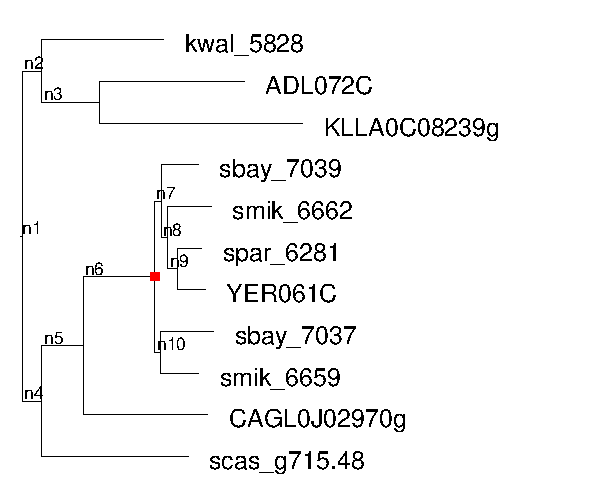
\includegraphics[width=3.5in]{figures/gene-tree.pdf}
\end{minipage}

\end{center}

\caption{{\bf Example *.recon file.} The reconciliation file format
(left) specifies how all the nodes in a gene tree (right) map to the
nodes and branches in the species tree (see \figref{fig:stree}).
Notice that gene node ``n6'' (red dot) represents a duplication event
along species branch ``n5'' (shown \figref{fig:stree}).  The gene tree
and species tree have their own name space (``n5'' in the gene tree is
not the same as ``n5'' in the species tree).}
\label{fig:recon}
\end{figure}


%=============================================================================
\subsection{SPIMAP model parameters file format (*.params)}
\label{sec:file:params}

\spimap\ has several parameters for its substitution rates model.
These parameters are learned by the {\tt spimap-train-rates} program,
which saves the parameters in a custom {\tt *.params} file format
(\figref{fig:params}).  The {\tt spimap} program reads these
parameters using the ``-p'' option.  Most uses of \spimap\ do not
require understanding the contents of a {\tt *.params} file.

The {\tt *.params} file format is tab-delimited and each line is
processed one at a time.

If the first field of a line is the word ``baserate'', then the
remaining two fields are interpreted as floating point values
$\alpha_G$ and $\beta_G$, which are the two parameters, shape and
scale, of the inverse-gamma distributed gene-specific rate.  

If the first field of the line does not match ``baserate'', then the first
field indicates a species tree branch and the remaining two fields
are interpreted as floating point values $\alpha_i$ and $\beta_i$,
which are the two parameters, shape and scale, of the gamma distributed
species-specific rate.  Each branch is indicated by its more recent node.
Ancestral nodes are indicated by an integer, where are assigned in 
pretraversal order.


%=========================================
% PARAMS FIGURE
\begin{figure}
\begin{center}
\footnotesize
\begin{lstlisting}[frame=tblr]
baserate  6.98457288742   5.98457288742
1         3.28887700831   394.209221588
2         4.64684152603   551.109741211
3         1.13027572632   164.191940308
4         0.610769152641  75.0393371582
5         7.14405012131   927.631103516
6         2.96983885765   238.195861816
7         5.63683271408   632.264831543
8         0.974860072136  94.9837493896
9         0.856632292271  78.6899032593
10        4.64683914185   544.528686523
11        1.92581880093   271.891052246
12        3.84569692612   624.703308105
13        3.14617466927   335.446655273
14        0.699178874493  84.1814575195
15        0.746283352375  137.345901489
scer      8.42576217651   763.305847168
ctro      6.70220327377   999.845153809
scas      9.14448356628   1253.45031738
agos      8.84074497223   801.648925781
sbay      6.95680332184   1048.7590332
kwal      14.3321857452   1962.9083252
dhan      15.7483224869   2699.00878906
smik      10.2562847137   1143.78076172
cgla      9.81903266907   1015.43951416
spar      5.80616807938   799.18963623
calb      8.38038921356   1233.68322754
lelo      9.40990924835   973.772583008
cpar      9.43262672424   1184.28100586
klac      6.6709280014    767.418823242
clus      8.37989234924   881.762878418
cgui      11.9692239761   1187.47314453
\end{lstlisting}


\end{center}

\caption{{\bf Example *.params file.}  The {\tt *.params} file contains the
parameters for \spimap's substitution rate model.}
\label{fig:params}
\end{figure}




%=============================================================================
%\clearpage
%raggedright
%\setstretch{1} 
%\bibliography{spimap-manual}

\end{document}
